\documentclass[border=3pt,tikz]{standalone}
\usepackage{tikz}
\usetikzlibrary{matrix,chains,positioning,decorations.pathreplacing,arrows}
\newcommand{\boldx}{ {\mathbf x} }
\begin{document}


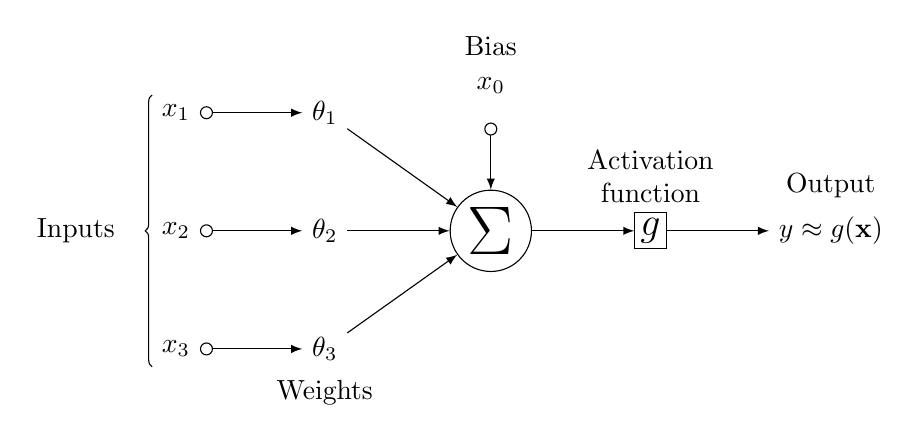
\begin{tikzpicture}[
init/.style={
  draw,
  circle,
  inner sep=2pt,
  font=\Huge,
  join = by -latex
},
squa/.style={
  draw,
  inner sep=2pt,
  font=\Large,
  join = by -latex
},
start chain=2,node distance=13mm
]
\node[on chain=2] 
  (theta2) {$x_2$};
\node[on chain=2,join=by o-latex] 
  {$\theta_2$};
\node[on chain=2,init] (sigma) 
  {$\displaystyle\Sigma$};
\node[on chain=2,squa,label=above:{\parbox{2cm}{\centering Activation \\ function}}]   
  {$g$};
\node[on chain=2,label=above:Output,join=by -latex] 
  {$y \approx g( \boldx)$};
\begin{scope}[start chain=1]
\node[on chain=1] at (0,1.5cm) 
  (x1) {$x_1$};
\node[on chain=1,join=by o-latex] 
  (theta1) {$\theta_1$};
\end{scope}
\begin{scope}[start chain=3]
\node[on chain=3] at (0,-1.5cm) 
  (x3) {$x_3$};
\node[on chain=3,label=below:Weights,join=by o-latex] 
  (theta3) {$\theta_3$};
\end{scope}
\node[label=above:\parbox{2cm}{\centering Bias \\ $x_0$}] at (sigma|-theta1) (x0) {};

\draw[-latex] (theta1) -- (sigma);
\draw[-latex] (theta3) -- (sigma);
\draw[o-latex] (x0) -- (sigma);

\draw[decorate,decoration={brace,mirror}] (x1.north west) -- node[left=10pt] {Inputs} (x3.south west);
\end{tikzpicture}

\end{document}